% ============================================================
% TFM -- Defensa académica
% "Procesamiento de datos en streaming y batch con
%  arquitecturas basadas en flujos de eventos"
% Gary Gianpier Choque Borda & Arthur Davis Huayaconza Condori
% UNIR -- Master Visual Analytics and Big Data -- Enero 2026
%
% Compilar: xelatex presentation.tex  (dos pasadas)
% ============================================================
\documentclass[aspectratio=169, 10pt]{beamer}
\usetheme{Madrid}

% ----------------------------------------------------------
% Fuentes (XeLaTeX)
% ----------------------------------------------------------
\usepackage{fontspec}
\setmainfont{DejaVu Sans}
\setsansfont{DejaVu Sans}
\setmonofont{DejaVu Sans Mono}

% ----------------------------------------------------------
% Paquetes
% ----------------------------------------------------------
\usepackage{tikz}
\usetikzlibrary{shapes.geometric, arrows.meta, positioning,
                fit, backgrounds, calc}
\usepackage{graphicx}
\usepackage{booktabs}
\usepackage{array}
\usepackage{multirow}
\usepackage{colortbl}
\usepackage{xcolor}
\usepackage{hyperref}
\usepackage{pgfplots}
\pgfplotsset{compat=1.18}

% ----------------------------------------------------------
% Colores corporativos UNIR
% ----------------------------------------------------------
\definecolor{unirblue}{HTML}{007CC0}
\definecolor{unirlightblue}{HTML}{4AAFD5}
\definecolor{unirdarkblue}{HTML}{005A8E}
\definecolor{uniraccent}{HTML}{E8F4FD}
\definecolor{successgreen}{HTML}{27AE60}
\definecolor{warningorange}{HTML}{E67E22}
\definecolor{alertred}{HTML}{C0392B}
\definecolor{kafkared}{HTML}{CC3333}
\definecolor{beamblue}{HTML}{2980B9}
\definecolor{mongodarkgreen}{HTML}{13AA52}
\definecolor{lightgray}{HTML}{F5F5F5}
\definecolor{darkgray}{HTML}{555555}
\definecolor{titlebg}{HTML}{005A8E}

% ----------------------------------------------------------
% Tema de colores personalizado UNIR
% ----------------------------------------------------------
\setbeamercolor{palette primary}{bg=unirdarkblue, fg=white}
\setbeamercolor{palette secondary}{bg=unirblue, fg=white}
\setbeamercolor{palette tertiary}{bg=unirlightblue, fg=white}
\setbeamercolor{palette quaternary}{bg=uniraccent, fg=unirdarkblue}
\setbeamercolor{structure}{fg=unirblue}
\setbeamercolor{title}{bg=unirdarkblue, fg=white}
\setbeamercolor{frametitle}{bg=unirblue, fg=white}
\setbeamercolor{block title}{bg=unirdarkblue, fg=white}
\setbeamercolor{block body}{bg=uniraccent, fg=black}
\setbeamercolor{block title alerted}{bg=alertred, fg=white}
\setbeamercolor{block body alerted}{bg=red!5, fg=black}
\setbeamercolor{block title example}{bg=successgreen, fg=white}
\setbeamercolor{block body example}{bg=green!5, fg=black}
\setbeamercolor{section in toc}{fg=unirdarkblue}
\setbeamercolor{itemize item}{fg=unirblue}
\setbeamercolor{itemize subitem}{fg=unirlightblue}
\setbeamerfont{frametitle}{size=\normalsize, series=\bfseries}

% ----------------------------------------------------------
% Estilos TikZ reutilizables
% ----------------------------------------------------------
\tikzset{
  box/.style={
    rectangle, rounded corners=3pt, draw=#1, fill=#1!15,
    text width=2.4cm, align=center, minimum height=0.9cm,
    font=\footnotesize\bfseries
  },
  wbox/.style={
    rectangle, rounded corners=3pt, draw=#1, fill=#1!15,
    align=center, minimum height=0.8cm,
    font=\footnotesize\bfseries
  },
  arrow/.style={-Stealth, thick, #1},
  stage/.style={
    rectangle, rounded corners=4pt, draw=unirblue, fill=unirblue!12,
    text width=1.8cm, align=center, minimum height=0.85cm,
    font=\scriptsize\bfseries
  },
  dlqbox/.style={
    rectangle, rounded corners=3pt, draw=alertred, fill=alertred!10,
    align=center, minimum height=0.8cm, font=\scriptsize\bfseries
  },
  techbox/.style={
    rectangle, rounded corners=4pt, draw=#1, fill=#1!12,
    align=center, minimum height=1.0cm, text width=2.2cm,
    font=\footnotesize\bfseries
  }
}

% ----------------------------------------------------------
% Pie de página personalizado
% ----------------------------------------------------------
\setbeamertemplate{footline}{%
  \leavevmode%
  \hbox{%
    \begin{beamercolorbox}[wd=.55\paperwidth, ht=2.5ex, dp=1.25ex,
        leftskip=4pt plus1fill, rightskip=4pt]{palette primary}%
      \usebeamerfont{author in head/foot}%
      G. Choque Borda \& A. Huayaconza Condori \;|\; TFM -- Arquitectura Dataflow
    \end{beamercolorbox}%
    \begin{beamercolorbox}[wd=.45\paperwidth, ht=2.5ex, dp=1.25ex,
        leftskip=4pt, rightskip=4pt plus1fill]{palette quaternary}%
      \usebeamerfont{date in head/foot}%
      \insertshorttitle \hfill \insertframenumber\,/\,\inserttotalframenumber
    \end{beamercolorbox}%
  }%
}
\setbeamertemplate{navigation symbols}{}

% ----------------------------------------------------------
% Metadatos
% ----------------------------------------------------------
\title[Arquitectura Dataflow]{%
  Procesamiento de datos en streaming y batch\\
  con arquitecturas basadas en flujos de eventos}
\subtitle{Trabajo Fin de Master}
\author{Gary Gianpier Choque Borda \and Arthur Davis Huayaconza Condori}
\institute{%
  Master Universitario en An\'alisis y Visualizaci\'on de Datos Masivos\\
  Visual Analytics and Big Data -- UNIR\\[4pt]
  Directora: Margalida Salom Ramis}
\date{Enero 2026}

% ============================================================
\begin{document}
% ============================================================

% ----------------------------------------------------------
% SLIDE 1 -- Portada
% ----------------------------------------------------------
\begin{frame}[plain]
  \begin{tikzpicture}[remember picture, overlay]
    % Fondo superior
    \fill[unirdarkblue]
      (current page.north west) rectangle
      ([yshift=-0.45\paperheight] current page.north east);
    % Banda inferior
    \fill[unirlightblue!30]
      ([yshift=-0.45\paperheight] current page.north west) rectangle
      (current page.south east);
    % Logo UNIR
    \node[anchor=north east] at
      ([xshift=-10pt, yshift=-8pt] current page.north east) {%
      
\includegraphics[height=1.0cm]{../doc_tfm/images/logo-unir.png}};
    % Título principal
    \node[anchor=center, text width=0.85\paperwidth, align=center] at
      ([yshift=0.10\paperheight] current page.center) {%
      {\color{white}\Large\bfseries
        Procesamiento de datos en streaming y batch\\[4pt]
        con arquitecturas basadas en flujos de eventos}\\[10pt]
      {\color{unirlightblue!80}\normalsize Trabajo Fin de Master}};
    % Autores
    \node[anchor=center, text width=0.85\paperwidth, align=center] at
      ([yshift=-0.02\paperheight] current page.center) {%
      {\color{unirdarkblue}\normalsize\bfseries
        Gary Gianpier Choque Borda \quad|\quad
        Arthur Davis Huayaconza Condori}\\[4pt]
      {\color{darkgray}\small
        Directora: Margalida Salom Ramis}};
    % Datos master
    \node[anchor=center, text width=0.85\paperwidth, align=center] at
      ([yshift=-0.14\paperheight] current page.center) {%
      {\color{darkgray}\small
        Master Universitario en An\'alisis y Visualizaci\'on de Datos Masivos\\
        Visual Analytics and Big Data -- UNIR \quad|\quad Enero 2026}};
  \end{tikzpicture}
\end{frame}

% ----------------------------------------------------------
% SLIDE 2 -- Índice
% ----------------------------------------------------------
\begin{frame}{\'Indice de contenidos}
  \begin{columns}[t]
    \column{0.48\textwidth}
      \tableofcontents[sections={1-7}, hideallsubsections]
    \column{0.48\textwidth}
      \tableofcontents[sections={8-13}, hideallsubsections]
  \end{columns}
\end{frame}

% ============================================================
\section{Motivaci\'on y Contexto}
% ============================================================

% ----------------------------------------------------------
% SLIDE 3 -- El problema: batch vs streaming
% ----------------------------------------------------------
\begin{frame}{El desaf\'io: batch vs.\ streaming}
  \begin{columns}[c]
    \column{0.45\textwidth}
      \includegraphics[width=\textwidth, keepaspectratio]%
        {../doc_tfm/images/batch-vs-stream.png}
    \column{0.52\textwidth}
      \begin{block}{Procesamiento batch}
        \begin{itemize}\setlength\itemsep{2pt}
          \item Datos hist\'oricos acumulados
          \item Alta latencia (horas/d\'ias)
          \item Resultados correctos pero tardos
        \end{itemize}
      \end{block}
      \vspace{6pt}
      \begin{alertblock}{Procesamiento en streaming}
        \begin{itemize}\setlength\itemsep{2pt}
          \item Datos en tiempo real
          \item Baja latencia (ms/s)
          \item Reto: datos tard\'ios y desordenados
        \end{itemize}
      \end{alertblock}
      \vspace{6pt}
      \begin{exampleblock}{La brecha}
        \small Las organizaciones necesitan \textbf{ambos modos} con una
        \'unica l\'ogica de negocio. Las arquitecturas cl\'asicas
        los tratan como sistemas separados.
      \end{exampleblock}
  \end{columns}
\end{frame}

% ----------------------------------------------------------
% SLIDE 4 -- Contexto epidemiológico
% ----------------------------------------------------------
\begin{frame}{Contexto: vigilancia epidemiol\'ogica COVID-19}
  \begin{columns}[c]
    \column{0.52\textwidth}
      \begin{block}{El caso real}
        \begin{itemize}\setlength\itemsep{3pt}
          \item Per\'u registr\'o millones de casos COVID-19
          \item Datos p\'ublicos del MINSA en \texttt{datos.gob.pe}
          \item 39 archivos CSV con 3 schemas distintos
          \item Necesidad de vigilancia \textbf{en tiempo real} y
                an\'alisis hist\'orico \textbf{unificados}
        \end{itemize}
      \end{block}
      \vspace{8pt}
      \begin{alertblock}{Desaf\'io de datos}
        \begin{itemize}\setlength\itemsep{2pt}
          \item Datos tard\'ios: reportes con d\'ias de retraso
          \item Schemas heterog\'eneos (9--54 campos)
          \item Registros inv\'alidos o incompletos
        \end{itemize}
      \end{alertblock}
    \column{0.44\textwidth}
      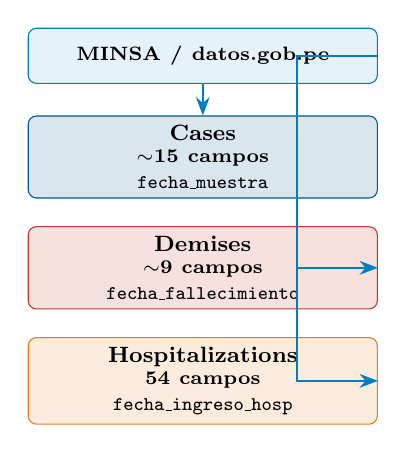
\begin{tikzpicture}
        \node[wbox=unirdarkblue, text width=4.2cm,
              minimum height=1.0cm] (cases)
          {\textbf{Cases}\\
           \scriptsize $\sim$15 campos\\
           \scriptsize \texttt{fecha\_muestra}};
        \node[wbox=alertred, text width=4.2cm,
              minimum height=1.0cm, below=0.35cm of cases] (demises)
          {\textbf{Demises}\\
           \scriptsize $\sim$9 campos\\
           \scriptsize \texttt{fecha\_fallecimiento}};
        \node[wbox=warningorange, text width=4.2cm,
              minimum height=1.0cm, below=0.35cm of demises] (hosp)
          {\textbf{Hospitalizations}\\
           \scriptsize 54 campos\\
           \scriptsize \texttt{fecha\_ingreso\_hosp}};
        \node[wbox=unirblue, text width=4.2cm,
              minimum height=0.7cm, above=0.4cm of cases,
              fill=unirblue!10] (src)
          {\scriptsize MINSA / datos.gob.pe};
        \draw[arrow=unirblue] (src) -- (cases);
        \draw[arrow=unirblue] (src) -- ++(1.2,0) |- (demises);
        \draw[arrow=unirblue] (src) -- ++(1.2,0) |- (hosp);
      \end{tikzpicture}
  \end{columns}
\end{frame}

% ============================================================
\section{Estado del Arte}
% ============================================================

% ----------------------------------------------------------
% SLIDE 5 -- Arquitectura Lambda
% ----------------------------------------------------------
\begin{frame}{Estado del arte: Arquitectura Lambda}
  \begin{columns}[c]
    \column{0.50\textwidth}
      \includegraphics[width=\textwidth, keepaspectratio]%
        {../doc_tfm/images/lambda-architecture.png}
    \column{0.46\textwidth}
      \begin{block}{Lambda Architecture (Nathan Marz, 2011)}
        \begin{itemize}\setlength\itemsep{3pt}
          \item \textbf{Batch layer}: reprocessa todo el historial
          \item \textbf{Speed layer}: procesa datos recientes
          \item \textbf{Serving layer}: combina ambas vistas
        \end{itemize}
      \end{block}
      \vspace{6pt}
      \begin{alertblock}{Limitaciones cr\'iticas}
        \begin{itemize}\setlength\itemsep{2pt}
          \item L\'ogica de negocio \textbf{duplicada} en batch y speed
          \item Mantenimiento costoso y propenso a errores
          \item Inconsistencias entre capas frecuentes
        \end{itemize}
      \end{alertblock}
  \end{columns}
\end{frame}

% ----------------------------------------------------------
% SLIDE 6 -- Arquitectura Kappa
% ----------------------------------------------------------
\begin{frame}{Estado del arte: Arquitectura Kappa}
  \begin{columns}[c]
    \column{0.50\textwidth}
      \includegraphics[width=\textwidth, keepaspectratio]%
        {../doc_tfm/images/kappa-architecture.png}
    \column{0.46\textwidth}
      \begin{block}{Kappa Architecture (Jay Kreps, 2014)}
        \begin{itemize}\setlength\itemsep{3pt}
          \item \textbf{Una sola capa}: todo como streaming
          \item L\'ogica unificada en un pipeline
          \item Reprocesamiento mediante replay del log
        \end{itemize}
      \end{block}
      \vspace{6pt}
      \begin{alertblock}{Limitaciones}
        \begin{itemize}\setlength\itemsep{2pt}
          \item Reprocesamiento masivo costoso en recursos
          \item Manejo de datos tard\'ios limitado
          \item Abstracci\'on insuficiente para event time
        \end{itemize}
      \end{alertblock}
  \end{columns}
\end{frame}

% ----------------------------------------------------------
% SLIDE 7 -- Comparativa de arquitecturas
% ----------------------------------------------------------
\begin{frame}[shrink=5]{Comparativa: Lambda vs.\ Kappa vs.\ \textbf{Dataflow}}
  \vspace{-4pt}
  \begin{center}
  \renewcommand{\arraystretch}{1.35}
  \begin{tabular}{>{\bfseries\small}l
                  >{\centering\arraybackslash\small}p{2.5cm}
                  >{\centering\arraybackslash\small}p{2.5cm}
                  >{\centering\arraybackslash\small}p{2.8cm}}
    \toprule
    \textbf{Criterio}
      & \textbf{Lambda}
      & \textbf{Kappa}
      & \textbf{\textcolor{unirdarkblue}{Dataflow}} \\
    \midrule
    L\'ogica unificada
      & \textcolor{alertred}{No}
      & \textcolor{successgreen}{S\'i}
      & \textcolor{successgreen}{\textbf{S\'i}} \\
    Datos tard\'ios (late data)
      & \textcolor{warningorange}{Parcial}
      & \textcolor{warningorange}{Parcial}
      & \textcolor{successgreen}{\textbf{Nativo}} \\
    Event time vs.\ processing time
      & \textcolor{alertred}{Processing}
      & \textcolor{warningorange}{Parcial}
      & \textcolor{successgreen}{\textbf{Event time}} \\
    Complejidad operacional
      & \textcolor{alertred}{Alta}
      & \textcolor{warningorange}{Media}
      & \textcolor{warningorange}{\textbf{Media}} \\
    Reutilizaci\'on de c\'odigo
      & \textcolor{alertred}{No}
      & \textcolor{successgreen}{S\'i}
      & \textcolor{successgreen}{\textbf{S\'i}} \\
    Abstracci\'on batch/stream
      & \textcolor{alertred}{No}
      & \textcolor{alertred}{No}
      & \textcolor{successgreen}{\textbf{PCollections}} \\
    Control de ventanas
      & \textcolor{alertred}{Limitado}
      & \textcolor{warningorange}{Parcial}
      & \textcolor{successgreen}{\textbf{Nativo}} \\
    \bottomrule
  \end{tabular}
  \end{center}
  \vspace{4pt}
  \begin{exampleblock}{}
    \centering\small
    El modelo \textbf{Dataflow} (Akidau et al., 2015) unifica semant\'icamente
    batch y streaming bajo una \'unica abstracci\'on, superando las limitaciones
    de sus predecesores.
  \end{exampleblock}
\end{frame}

% ============================================================
\section{El Modelo Dataflow}
% ============================================================

% ----------------------------------------------------------
% SLIDE 8 -- PCollections y modelo de programación
% ----------------------------------------------------------
\begin{frame}{Modelo Dataflow: PCollections y Apache Beam}
  \begin{columns}[c]
    \column{0.50\textwidth}
      \begin{block}{PCollections -- la abstracci\'on clave}
        \begin{itemize}\setlength\itemsep{3pt}
          \item Conjunto de datos \textbf{inmutable y potencialmente ilimitado}
          \item Mismo tipo representa batch \textit{y} stream
          \item Transformaciones mediante \texttt{PTransform}
          \item El runner decide c\'omo ejecutar
        \end{itemize}
      \end{block}
      \vspace{6pt}
      \begin{exampleblock}{Apache Beam}
        \small
        SDK open-source que implementa el modelo Dataflow.\\[4pt]
        \textbf{Runners:} Direct, Flink, Spark, Dataflow (GCP)\\[4pt]
        En este TFM: \textbf{DirectRunner} (local, reproducible)
      \end{exampleblock}
    \column{0.46\textwidth}
      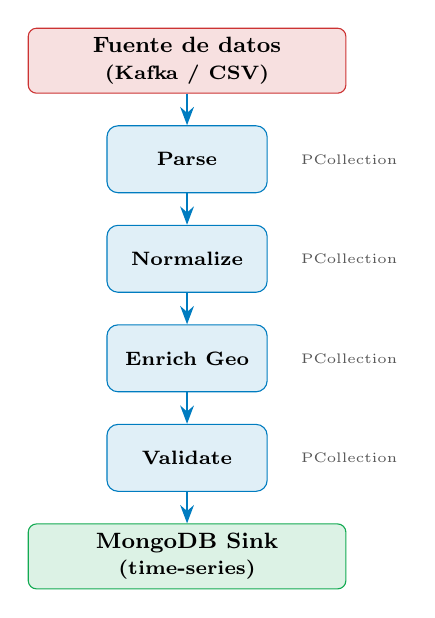
\begin{tikzpicture}[node distance=0.55cm]
        \node[wbox=kafkared, text width=3.8cm] (src)
          {Fuente de datos\\
           \scriptsize (Kafka / CSV)};
        \node[stage, below=0.4cm of src] (p1) {Parse};
        \node[stage, below=0.4cm of p1] (p2) {Normalize};
        \node[stage, below=0.4cm of p2] (p3) {Enrich Geo};
        \node[stage, below=0.4cm of p3] (p4) {Validate};
        \node[wbox=mongodarkgreen, text width=3.8cm,
              below=0.4cm of p4] (sink)
          {MongoDB Sink\\
           \scriptsize (time-series)};
        \foreach \a/\b in {src/p1, p1/p2, p2/p3, p3/p4, p4/sink}{%
          \draw[arrow=unirblue] (\a) -- (\b);}
        \node[right=0.3cm of p1, font=\tiny, text=darkgray]
          {PCollection};
        \node[right=0.3cm of p2, font=\tiny, text=darkgray]
          {PCollection};
        \node[right=0.3cm of p3, font=\tiny, text=darkgray]
          {PCollection};
        \node[right=0.3cm of p4, font=\tiny, text=darkgray]
          {PCollection};
      \end{tikzpicture}
  \end{columns}
\end{frame}

% ----------------------------------------------------------
% SLIDE 9 -- Event time, Watermarks y Windows
% ----------------------------------------------------------
\begin{frame}{Modelo Dataflow: Event Time, Watermarks y Windows}
  \begin{columns}[t]
    \column{0.48\textwidth}
      \begin{block}{Event time vs.\ Processing time}
        \begin{itemize}\setlength\itemsep{2pt}
          \item \textbf{Event time}: cu\'ando ocurri\'o el evento real
          \item \textbf{Processing time}: cu\'ando llega al sistema
          \item El Dataflow model trabaja sobre \textbf{event time}
          \item Garantiza resultados correctos incluso con retrasos
        \end{itemize}
      \end{block}
      \vspace{4pt}
      \begin{block}{Watermarks}
        \small
        Se\~nal de progreso temporal: ``todos los eventos con
        event time $<$ W han llegado''. Permite \textbf{cerrar ventanas}
        de forma determinista.
      \end{block}
    \column{0.48\textwidth}
      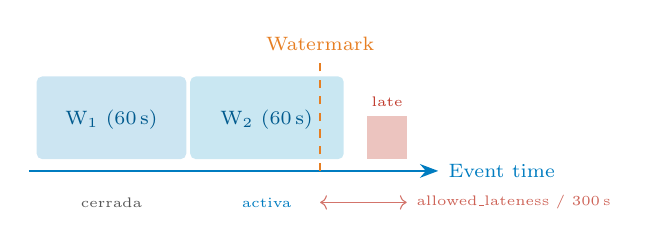
\begin{tikzpicture}
        % Eje tiempo
        \draw[thick, -Stealth, unirblue] (0,0) -- (5.2,0)
          node[right, font=\scriptsize] {Event time};
        % Ventanas
        \fill[unirblue!20, rounded corners=2pt]
          (0.1,0.15) rectangle (2.0,1.2);
        \fill[unirlightblue!30, rounded corners=2pt]
          (2.05,0.15) rectangle (4.0,1.2);
        \node[font=\scriptsize, unirdarkblue] at (1.05,0.65)
          {W$_1$ (60\,s)};
        \node[font=\scriptsize, unirdarkblue] at (3.02,0.65)
          {W$_2$ (60\,s)};
        % Late data
        \fill[alertred!30] (4.3,0.15) rectangle (4.8,0.7);
        \node[font=\tiny, alertred, above] at (4.55,0.7)
          {late};
        % Watermark
        \draw[dashed, thick, warningorange] (3.7,0) -- (3.7,1.4)
          node[above, font=\scriptsize, text=warningorange]
          {Watermark};
        % allowed lateness
        \draw[<->, alertred!70] (3.7,-0.4) -- (4.8,-0.4)
          node[right, font=\tiny, text=alertred!80]
          {allowed\_lateness / 300\,s};
        % Labels
        \node[font=\tiny, darkgray] at (1.05,-0.4) {cerrada};
        \node[font=\tiny, unirblue] at (3.02,-0.4) {activa};
      \end{tikzpicture}
      \vspace{4pt}
      \begin{exampleblock}{\small Configuraci\'on en este TFM}
        \scriptsize
        Ventanas fijas: \textbf{60 s}\\
        Allowed lateness: \textbf{300 s} (5 min)\\
        Trigger: \texttt{AfterWatermark} + \texttt{AfterProcessingTime}
      \end{exampleblock}
  \end{columns}
\end{frame}

% ----------------------------------------------------------
% SLIDE 10 -- Triggers
% ----------------------------------------------------------
\begin{frame}{Modelo Dataflow: Triggers}
  \begin{columns}[c]
    \column{0.50\textwidth}
      \begin{block}{?`Qu\'e es un trigger?}
        \small
        Controla \textbf{cu\'ando} se emiten los resultados de una ventana.
        Permite ver resultados parciales antes de que la ventana cierre.
      \end{block}
      \vspace{6pt}
      \begin{block}{Tipos de trigger principales}
      \renewcommand{\arraystretch}{1.3}
      \begin{tabular}{>{\small}l >{\small}p{3.2cm}}
        \toprule
        \textbf{Trigger} & \textbf{Cu\'ando emite} \\
        \midrule
        AfterWatermark & Al cruzar el watermark \\
        AfterProcessingTime & Tras N segundos \\
        AfterCount & Al acumular N elementos \\
        Repeat & Repite cualquier trigger \\
        \bottomrule
      \end{tabular}
      \end{block}
    \column{0.46\textwidth}
      \begin{exampleblock}{Configuraci\'on en el TFM}
        \footnotesize
        \texttt{\textbf{AfterWatermark}}\\
        \hspace{8pt}\texttt{.past\_end\_of\_window()}\\
        \hspace{4pt}\texttt{.with\_early\_firings(}\\
        \hspace{8pt}\texttt{AfterProcessingTime}\\
        \hspace{10pt}\texttt{.of(30)}\\
        \hspace{4pt}\texttt{)}\\
        \hspace{4pt}\texttt{.with\_late\_firings(}\\
        \hspace{8pt}\texttt{AfterCount(1)}\\
        \hspace{4pt}\texttt{)}
      \end{exampleblock}
      \vspace{6pt}
      \begin{alertblock}{\small Resultado}
        \small
        Emisi\'on \textbf{temprana} cada 30\,s (vista preliminar),
        emisi\'on \textbf{final} al cerrar ventana,
        emisi\'on adicional por cada dato tard\'io recibido.
      \end{alertblock}
  \end{columns}
\end{frame}

% ============================================================
\section{Objetivos y Metodolog\'ia}
% ============================================================

% ----------------------------------------------------------
% SLIDE 11 -- Objetivos
% ----------------------------------------------------------
\begin{frame}{Objetivos del TFM}
  \begin{columns}[t]
    \column{0.48\textwidth}
      \begin{block}{Objetivo general}
        \small
        Dise\~nar e implementar un sistema de procesamiento de datos
        epidemiol\'ogicos que unifique batch y streaming mediante el
        \textbf{modelo Dataflow} sobre datos COVID-19 reales del MINSA Per\'u.
      \end{block}
      \vspace{6pt}
      \begin{exampleblock}{OE1 -- Arquitectura Dataflow}
        \small Implementar pipeline Apache Beam con PCollections,
        watermarks, windows y triggers.
      \end{exampleblock}
      \begin{exampleblock}{OE2 -- Broker de mensajes}
        \small Integrar Apache Kafka como capa de desacoplamiento
        entre ingesta y procesamiento.
      \end{exampleblock}
      \begin{exampleblock}{OE3 -- Almacenamiento time-series}
        \small Persistir resultados en MongoDB con colecciones
        time-series optimizadas.
      \end{exampleblock}
    \column{0.48\textwidth}
      \begin{exampleblock}{OE4 -- Extensibilidad de schemas}
        \small Dise\~nar arquitectura modular para a\~nadir nuevos
        schemas con m\'inimo esfuerzo.
      \end{exampleblock}
      \begin{exampleblock}{OE5 -- Dashboard en tiempo real}
        \small Visualizaciones interactivas con D3.js y Leaflet.js
        actualizadas via WebSockets.
      \end{exampleblock}
      \begin{exampleblock}{OE6 -- Evaluaci\'on y validaci\'on}
        \small Medir latencia, throughput y coherencia en 4 escenarios
        de prueba distintos.
      \end{exampleblock}
      \vspace{6pt}
      \begin{alertblock}{}
        \centering\small\bfseries
        6/6 objetivos espec\'ificos completados al 100\,\%
      \end{alertblock}
  \end{columns}
\end{frame}

% ----------------------------------------------------------
% SLIDE 12 -- Metodología
% ----------------------------------------------------------
\begin{frame}{Metodolog\'ia: CRISP-DM + Kanban}
  \begin{columns}[c]
    \column{0.50\textwidth}
      \begin{block}{CRISP-DM adaptado}
        \begin{itemize}\setlength\itemsep{2pt}
          \item \textbf{Business Understanding}: vigilancia epidemiol\'ogica
          \item \textbf{Data Understanding}: 3 schemas MINSA, 39 CSVs
          \item \textbf{Data Preparation}: normalizaci\'on, enriquecimiento geo
          \item \textbf{Modeling}: pipeline Beam + ventanas temporales
          \item \textbf{Evaluation}: 4 escenarios de prueba
          \item \textbf{Deployment}: Docker Compose reproducible
        \end{itemize}
      \end{block}
    \column{0.46\textwidth}
      \begin{block}{Gesti\'on con Kanban}
        \begin{itemize}\setlength\itemsep{3pt}
          \item Tablero visual con columnas:\\
                Backlog $\to$ En progreso $\to$ Hecho
          \item Iteraciones cortas de 1--2 semanas
          \item Priorizaci\'on continua de tareas
          \item Colaboraci\'on distribuida (2 autores)
        \end{itemize}
      \end{block}
      \vspace{6pt}
      \begin{exampleblock}{Herramientas}
        \small
        GitHub + Docker + Python + XeLaTeX\\
        Testing manual en 4 escenarios documentados
      \end{exampleblock}
  \end{columns}
\end{frame}

% ============================================================
\section{Caso de Uso: COVID-19 Per\'u}
% ============================================================

% ----------------------------------------------------------
% SLIDE 13 -- Datos MINSA
% ----------------------------------------------------------
\begin{frame}{Caso de uso: Datos COVID-19 MINSA Per\'u}
  \begin{columns}[c]
    \column{0.50\textwidth}
      \begin{block}{Fuente de datos}
        \begin{itemize}\setlength\itemsep{2pt}
          \item \textbf{Origen}: datos.gob.pe (MINSA Per\'u)
          \item Datos reales anonimizados
          \item \textbf{39 archivos CSV} con millones de registros
          \item Tres schemas con estructuras heterog\'eneas
          \item Lectura eficiente con \textbf{Polars}
        \end{itemize}
      \end{block}
      \vspace{4pt}
      \begin{alertblock}{Retos de los datos}
        \begin{itemize}\setlength\itemsep{2pt}
          \item Valores nulos y formatos inconsistentes
          \item UBIGEO (c\'odigo geogr\'afico peruano) sin coordenadas
          \item Fechas en formato \texttt{YYYYMMDD} no est\'andar
          \item Datos tard\'ios: reportes con varios d\'ias de retraso
        \end{itemize}
      \end{alertblock}
    \column{0.46\textwidth}
      \renewcommand{\arraystretch}{1.4}
      \begin{tabular}{>{\bfseries\small}l
                      >{\centering\arraybackslash\small}c
                      >{\small}l}
        \toprule
        Schema & Campos & Timestamp \\
        \midrule
        \textcolor{unirdarkblue}{Cases}
          & $\sim$15
          & \texttt{\scriptsize fecha\_muestra} \\
        \textcolor{alertred}{Demises}
          & $\sim$9
          & \texttt{\scriptsize fecha\_fallecimiento} \\
        \textcolor{warningorange}{Hospitalizations}
          & 54
          & \texttt{\scriptsize fecha\_ingreso\_hosp} \\
        \bottomrule
      \end{tabular}
      \vspace{8pt}
      \begin{exampleblock}{Enriquecimiento geogr\'afico}
        \small
        Cada registro incluye c\'odigo UBIGEO.\\
        El pipeline enriquece con:
        latitud, longitud, departamento, provincia,
        distrito -- habilitando los mapas de calor.
      \end{exampleblock}
  \end{columns}
\end{frame}

% ----------------------------------------------------------
% SLIDE 14 -- Schema Cases
% ----------------------------------------------------------
\begin{frame}[shrink=8]{Detalle de schemas: campos principales}
  \begin{columns}[t]
    \column{0.32\textwidth}
      \begin{block}{\textcolor{unirdarkblue}{Cases} ($\sim$15 campos)}
        \scriptsize
        \texttt{UUID}, \texttt{DEPARTAMENTO}\\
        \texttt{PROVINCIA}, \texttt{DISTRITO}\\
        \texttt{METODODX} (tipo de prueba)\\
        \texttt{EDAD}, \texttt{SEXO}\\
        \texttt{FECHA\_RESULTADO}\\
        \texttt{UBIGEO}, \texttt{id\_persona}\\[3pt]
        \textbf{Timestamp}: \texttt{fecha\_muestra}
      \end{block}
    \column{0.32\textwidth}
      \begin{block}{\textcolor{alertred}{Demises} ($\sim$9 campos)}
        \scriptsize
        \texttt{UUID}, \texttt{EDAD\_DECLARADA}\\
        \texttt{SEXO}, \texttt{DEPARTAMENTO}\\
        \texttt{PROVINCIA}, \texttt{DISTRITO}\\
        \texttt{UBIGEO}\\[3pt]
        \textbf{Timestamp}: \texttt{fecha\_fallecimiento}
      \end{block}
    \column{0.32\textwidth}
      \begin{block}{\textcolor{warningorange}{Hospitalizations} (54 campos)}
        \scriptsize
        \texttt{id\_persona}, \texttt{UBIGEO}\\
        \texttt{SEXO}, \texttt{EDAD}\\
        \texttt{UCI} (booleano)\\
        \texttt{VENTILACION} (booleano)\\
        \texttt{VACUNA1}, \texttt{VACUNA2}, \texttt{VACUNA3}\\
        \texttt{flag\_uci}, \texttt{n\_dias\_hosp}\\
        \ldots\ (+44 campos m\'as)\\[3pt]
        \textbf{Timestamp}: \texttt{fecha\_ingreso\_hosp}
      \end{block}
  \end{columns}
  \vspace{6pt}
  \begin{exampleblock}{Kafka Topics}
    \centering\small
    \textbf{topic:} \texttt{cases} \quad|\quad
    \textbf{topic:} \texttt{demises} \quad|\quad
    \textbf{topic:} \texttt{hospitalizations}\\[2pt]
    Cada topic corresponde a un schema y alimenta su propio pipeline paralelo.
  \end{exampleblock}
\end{frame}

% ----------------------------------------------------------
% SLIDE 15 -- Flujo de datos completo (imagen)
% ----------------------------------------------------------
\begin{frame}{Flujo de datos de extremo a extremo}
  \begin{center}
    \includegraphics[height=0.75\textheight, keepaspectratio]%
      {../doc_tfm/images/flujo-datos-completo.png}
  \end{center}
\end{frame}

% ============================================================
\section{Arquitectura del Sistema}
% ============================================================

% ----------------------------------------------------------
% SLIDE 16 -- Visión general de la arquitectura
% ----------------------------------------------------------
\begin{frame}{Arquitectura general del sistema}
  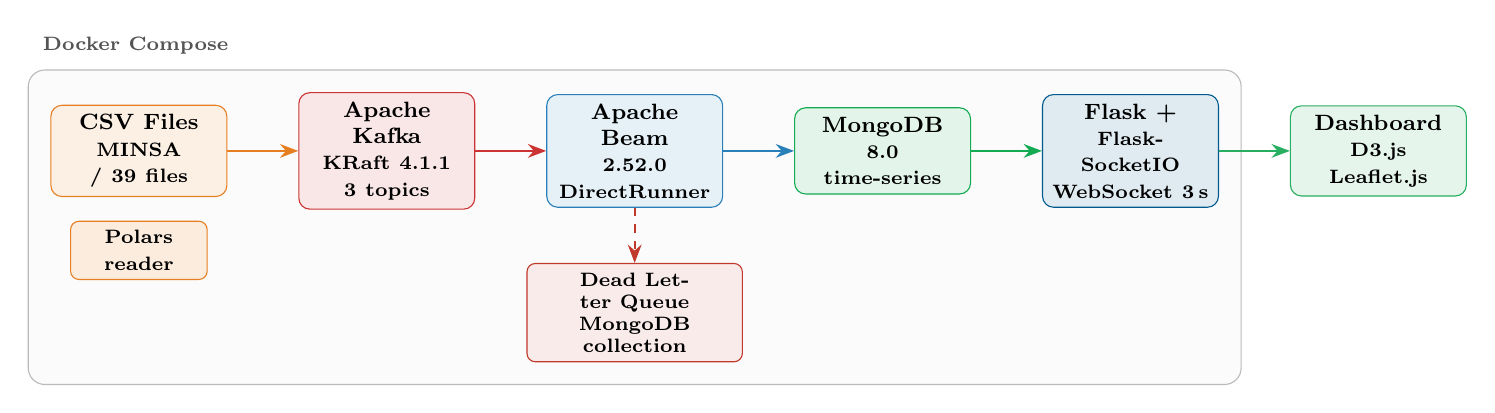
\begin{tikzpicture}[node distance=0.5cm and 0.6cm]
    % Ingesta
    \node[techbox=warningorange, text width=2.0cm] (csv)
      {CSV Files\\{\scriptsize MINSA / 39 files}};
    \node[wbox=warningorange, text width=1.5cm,
          below=0.3cm of csv, minimum height=0.7cm] (polars)
      {{\scriptsize Polars}\\{\scriptsize reader}};

    % Kafka
    \node[techbox=kafkared, text width=2.0cm,
          right=0.9cm of csv] (kafka)
      {Apache Kafka\\{\scriptsize KRaft 4.1.1}\\{\scriptsize 3 topics}};

    % Beam pipeline
    \node[techbox=beamblue, text width=2.0cm,
          right=0.9cm of kafka] (beam)
      {Apache Beam\\{\scriptsize 2.52.0}\\{\scriptsize DirectRunner}};

    % MongoDB
    \node[techbox=mongodarkgreen, text width=2.0cm,
          right=0.9cm of beam] (mongo)
      {MongoDB\\{\scriptsize 8.0}\\{\scriptsize time-series}};

    % Flask backend
    \node[techbox=unirdarkblue, text width=2.0cm,
          right=0.9cm of mongo] (flask)
      {Flask +\\{\scriptsize Flask-SocketIO}\\{\scriptsize WebSocket 3\,s}};

    % Dashboard
    \node[techbox=successgreen, text width=2.0cm,
          right=0.9cm of flask] (dash)
      {Dashboard\\{\scriptsize D3.js}\\{\scriptsize Leaflet.js}};

    % DLQ
    \node[dlqbox, text width=2.5cm,
          below=0.7cm of beam] (dlq)
      {Dead Letter Queue\\{\scriptsize MongoDB collection}};

    % Flechas principales
    \draw[arrow=warningorange] (csv) -- (kafka);
    \draw[arrow=kafkared] (kafka) -- (beam);
    \draw[arrow=beamblue] (beam) -- (mongo);
    \draw[arrow=mongodarkgreen] (mongo) -- (flask);
    \draw[arrow=successgreen] (flask) -- (dash);
    \draw[arrow=alertred, dashed] (beam) -- (dlq);

    % Docker Compose label
    \begin{scope}[on background layer]
      \node[rectangle, rounded corners=6pt,
            draw=darkgray, fill=lightgray, opacity=0.4,
            fit=(csv)(polars)(kafka)(beam)(mongo)(flask)(dlq),
            inner sep=8pt] (docker) {};
    \end{scope}
    \node[font=\scriptsize\bfseries, darkgray,
          above right=2pt and 2pt of docker.north west]
      {Docker Compose};
  \end{tikzpicture}
\end{frame}

% ----------------------------------------------------------
% SLIDE 17 -- Infraestructura Docker
% ----------------------------------------------------------
\begin{frame}{Infraestructura: Docker Compose}
  \begin{columns}[c]
    \column{0.50\textwidth}
      \begin{block}{Servicios en contenedores}
        \begin{itemize}\setlength\itemsep{3pt}
          \item \textbf{kafka}: broker KRaft (sin Zookeeper)
          \item \textbf{init-kafka}: crea topics al inicio
          \item \textbf{mongodb}: base de datos time-series
          \item \textbf{pipeline-cases}: pipeline + ingesta cases
          \item \textbf{pipeline-demises}: pipeline + ingesta demises
          \item \textbf{pipeline-hospitalizations}: pipeline + ingesta hosp.
          \item \textbf{dashboard}: Flask + WebSockets + D3.js
        \end{itemize}
      \end{block}
    \column{0.46\textwidth}
      \begin{exampleblock}{Ventajas del enfoque}
        \begin{itemize}\setlength\itemsep{3pt}
          \item Entorno \textbf{completamente reproducible}
          \item Un solo comando: \texttt{docker compose up}
          \item Red interna entre servicios
          \item F\'acil incorporaci\'on de nuevos pipelines
        \end{itemize}
      \end{exampleblock}
      \vspace{6pt}
      \begin{alertblock}{Paralelismo}
        \small
        Los 3 schemas procesan \textbf{en paralelo} en contenedores
        independientes, cada uno con su propio topic Kafka,
        instancia de pipeline Beam y colecci\'on MongoDB.
      \end{alertblock}
  \end{columns}
\end{frame}

% ----------------------------------------------------------
% SLIDE 18 -- Las 8 etapas del pipeline
% ----------------------------------------------------------
\begin{frame}{Pipeline Apache Beam: 8 etapas}
  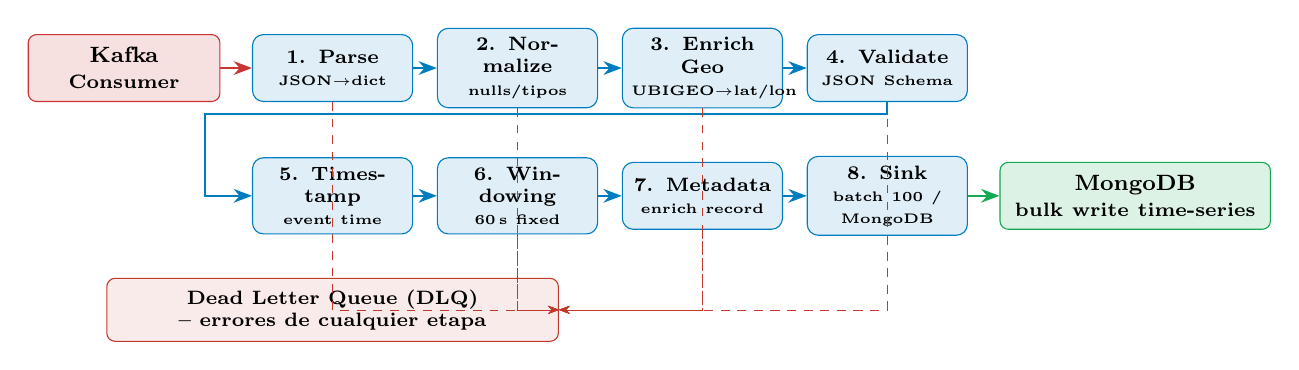
\begin{tikzpicture}[node distance=0.22cm and 0.05cm]
    % Stages en dos filas de 4
    \node[stage] (p1) {1. Parse\\{\tiny JSON$\to$dict}};
    \node[stage, right=0.3cm of p1] (p2) {2. Normalize\\{\tiny nulls/tipos}};
    \node[stage, right=0.3cm of p2] (p3) {3. Enrich Geo\\{\tiny UBIGEO$\to$lat/lon}};
    \node[stage, right=0.3cm of p3] (p4) {4. Validate\\{\tiny JSON Schema}};

    \node[stage, below=0.7cm of p1] (p5) {5. Timestamp\\{\tiny event time}};
    \node[stage, right=0.3cm of p5] (p6) {6. Windowing\\{\tiny 60\,s fixed}};
    \node[stage, right=0.3cm of p6] (p7) {7. Metadata\\{\tiny enrich record}};
    \node[stage, right=0.3cm of p7] (p8) {8. Sink\\{\tiny batch 100 / MongoDB}};

    % Flechas fila 1
    \foreach \a/\b in {p1/p2, p2/p3, p3/p4}{%
      \draw[arrow=unirblue] (\a) -- (\b);}
    % Bajada
    \draw[arrow=unirblue] (p4.south) -- ++(0,-0.15)
      -| ([xshift=-0.6cm]p5.west) -- (p5.west);
    % Flechas fila 2
    \foreach \a/\b in {p5/p6, p6/p7, p7/p8}{%
      \draw[arrow=unirblue] (\a) -- (\b);}

    % DLQ
    \node[dlqbox, below=0.55cm of p5, text width=5.5cm] (dlq)
      {Dead Letter Queue (DLQ) -- errores de cualquier etapa};
    \foreach \s in {p1,p2,p3,p4,p5,p6,p7,p8}{%
      \draw[arrow=alertred, dashed, very thin]
        (\s.south) -- ++(0,-0.1) |- (dlq.east);}

    % MongoDB sink
    \node[wbox=mongodarkgreen, text width=3.2cm,
          right=0.4cm of p8, minimum height=0.85cm] (mdb)
      {MongoDB\\{\scriptsize bulk write time-series}};
    \draw[arrow=mongodarkgreen] (p8) -- (mdb);

    % Kafka source
    \node[wbox=kafkared, text width=2.2cm,
          left=0.4cm of p1, minimum height=0.85cm] (kfk)
      {Kafka\\{\scriptsize Consumer}};
    \draw[arrow=kafkared] (kfk) -- (p1);
  \end{tikzpicture}

  \vspace{4pt}
  \begin{columns}[t]
    \column{0.48\textwidth}
      \begin{exampleblock}{\small Etapas 1--4: Preparaci\'on}
        \scriptsize
        \textbf{Parse}: string JSON a diccionario Python.
        \textbf{Normalize}: nulos a \texttt{None}, conversiones de tipo.
        \textbf{Enrich Geo}: c\'odigo UBIGEO a lat/lon.
        \textbf{Validate}: validaci\'on contra JSON Schema.
      \end{exampleblock}
    \column{0.48\textwidth}
      \begin{exampleblock}{\small Etapas 5--8: Procesamiento temporal}
        \scriptsize
        \textbf{Timestamp}: campo fecha a event time.
        \textbf{Windowing}: ventana fija 60\,s.
        \textbf{Metadata}: a\~nade \texttt{pipeline\_version},
        \texttt{source\_type}, \texttt{processed\_at}, info de ventana.
        \textbf{Sink}: batch de 100, bulk write.
      \end{exampleblock}
  \end{columns}
\end{frame}

% ----------------------------------------------------------
% SLIDE 19 -- Ventanas temporales en detalle
% ----------------------------------------------------------
\begin{frame}{Ventanas temporales y manejo de datos tard\'ios}
  \begin{columns}[c]
    \column{0.50\textwidth}
      \begin{block}{Configuraci\'on de windowing}
        \begin{itemize}\setlength\itemsep{3pt}
          \item \textbf{Tipo}: FixedWindows (60 segundos)
          \item \textbf{Allowed lateness}: 300 s (5 minutos)
          \item Datos que llegan dentro de la ventana: procesados
          \item Datos tard\'ios dentro del grace period: \textbf{re-agregados}
          \item Datos m\'as all\'a del grace: $\to$ \textbf{DLQ}
        \end{itemize}
      \end{block}
      \vspace{4pt}
      \begin{exampleblock}{Metadata de ventana}
        \scriptsize
        Cada registro guardado incluye:\\
        \texttt{window\_start}, \texttt{window\_end},\\
        \texttt{pipeline\_version}, \texttt{source\_type},\\
        \texttt{processed\_at}
      \end{exampleblock}
    \column{0.46\textwidth}
      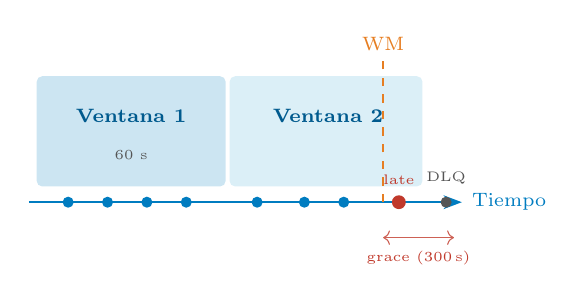
\begin{tikzpicture}
        \draw[thick,-Stealth, unirblue] (0,0) -- (5.5,0)
          node[right, font=\scriptsize] {Tiempo};
        % Ventana 1
        \fill[unirblue!20, rounded corners=2pt]
          (0.1,0.2) rectangle (2.5,1.6);
        \node[font=\scriptsize\bfseries, unirdarkblue]
          at (1.3,1.1) {Ventana 1};
        \node[font=\tiny, darkgray] at (1.3,0.6) {60 s};
        % Ventana 2
        \fill[unirlightblue!20, rounded corners=2pt]
          (2.55,0.2) rectangle (5.0,1.6);
        \node[font=\scriptsize\bfseries, unirdarkblue]
          at (3.8,1.1) {Ventana 2};
        % Watermark
        \draw[dashed, thick, warningorange]
          (4.5,0) -- (4.5,1.8)
          node[above, font=\scriptsize, text=warningorange] {WM};
        % Grace period
        \draw[<->, alertred!80] (4.5,-0.45) -- (5.4,-0.45);
        \node[font=\tiny, alertred, below] at (4.95,-0.5) {grace (300\,s)};
        % Eventos normales
        \foreach \x in {0.5,1.0,1.5,2.0,2.9,3.5,4.0}{%
          \fill[unirblue] (\x,0) circle (2pt);}
        % Late event
        \fill[alertred] (4.7,0) circle (2.5pt);
        \node[font=\tiny, alertred, above] at (4.7,0.1) {late};
        % DLQ event
        \fill[darkgray] (5.3,0) circle (2pt);
        \node[font=\tiny, darkgray, above] at (5.3,0.1) {DLQ};
      \end{tikzpicture}
  \end{columns}
\end{frame}

% ----------------------------------------------------------
% SLIDE 20 -- Dead Letter Queue y orquestador
% ----------------------------------------------------------
\begin{frame}{Dead Letter Queue y Orquestador de schemas}
  \begin{columns}[t]
    \column{0.50\textwidth}
      \begin{alertblock}{Dead Letter Queue (DLQ)}
        \begin{itemize}\setlength\itemsep{2pt}
          \item Captura errores de \textbf{todas} las etapas del pipeline
          \item Colecci\'on \texttt{dead\_letter\_queue} en MongoDB
          \item Campos almacenados:
            \begin{itemize}\setlength\itemsep{1pt}
              \item \texttt{error}: mensaje de error
              \item \texttt{error\_type}: tipo/etapa del fallo
              \item \texttt{timestamp}: momento del error
              \item \texttt{schema}: cases / demises / hosp
              \item \texttt{record}: registro original completo
            \end{itemize}
          \item Datos inv\'alidos \textbf{no bloquean} el pipeline
          \item Permite auditor\'ia y depuraci\'on post-facto
        \end{itemize}
      \end{alertblock}
    \column{0.46\textwidth}
      \begin{block}{Orquestador autom\'atico}
        \begin{itemize}\setlength\itemsep{3pt}
          \item Lee la carpeta \texttt{pipelines/}
          \item \textbf{Descubre schemas autom\'aticamente}
          \item Lanza cada pipeline en su propio proceso
          \item No requiere configuraci\'on manual al a\~nadir schemas
        \end{itemize}
      \end{block}
      \vspace{6pt}
      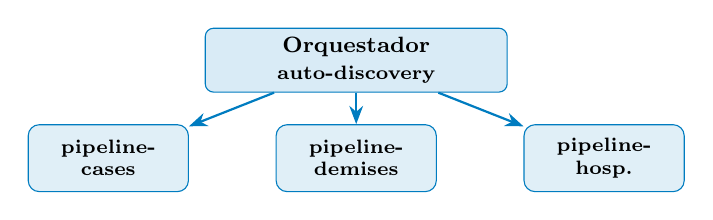
\begin{tikzpicture}[node distance=0.4cm]
        \node[wbox=unirblue, text width=3.6cm] (orch)
          {Orquestador\\{\scriptsize auto-discovery}};
        \node[stage, text width=1.8cm,
              below left=0.4cm and 0.2cm of orch] (pc)
          {pipeline-\\cases};
        \node[stage, text width=1.8cm,
              below=0.4cm of orch] (pd)
          {pipeline-\\demises};
        \node[stage, text width=1.8cm,
              below right=0.4cm and 0.2cm of orch] (ph)
          {pipeline-\\hosp.};
        \foreach \t in {pc,pd,ph}{%
          \draw[arrow=unirblue] (orch) -- (\t);}
      \end{tikzpicture}
  \end{columns}
\end{frame}

% ============================================================
\section{Extensibilidad del Sistema}
% ============================================================

% ----------------------------------------------------------
% SLIDE 21 -- Diseño modular
% ----------------------------------------------------------
\begin{frame}{Dise\~no modular: extensibilidad de schemas}
  \begin{columns}[c]
    \column{0.50\textwidth}
      \begin{block}{Principio de dise\~no}
        \small
        Toda la l\'ogica compartida reside en \texttt{src/common/}.
        Cada schema es un \textbf{plugin} que solo configura
        su nombre, topic y colecci\'on.
      \end{block}
      \vspace{4pt}
      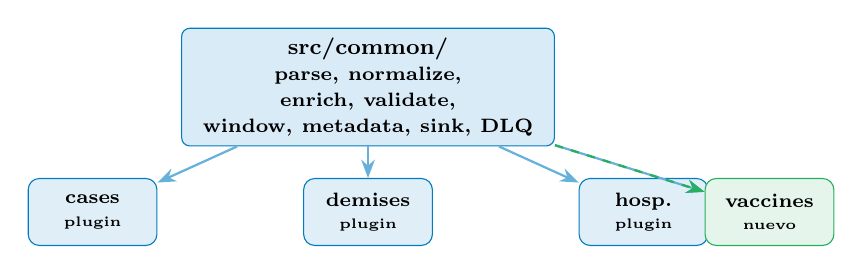
\begin{tikzpicture}[node distance=0.35cm]
        \node[wbox=unirblue, text width=4.5cm] (common)
          {\textbf{src/common/}\\
           {\scriptsize parse, normalize, enrich, validate,}\\
           {\scriptsize window, metadata, sink, DLQ}};
        \node[stage, text width=1.4cm,
              below left=0.4cm and 0.3cm of common] (sc)
          {cases\\{\tiny plugin}};
        \node[stage, text width=1.4cm,
              below=0.4cm of common] (sd)
          {demises\\{\tiny plugin}};
        \node[stage, text width=1.4cm,
              below right=0.4cm and 0.3cm of common] (sh)
          {hosp.\\{\tiny plugin}};
        \node[stage, text width=1.4cm, draw=successgreen,
              fill=successgreen!12,
              below right=0.4cm and 1.9cm of common] (sv)
          {vaccines\\{\tiny nuevo}};
        \foreach \t in {sc,sd,sh,sv}{%
          \draw[arrow=unirblue!60] (common) -- (\t);}
        \draw[arrow=successgreen, dashed] (common) -- (sv);
      \end{tikzpicture}
    \column{0.46\textwidth}
      \begin{exampleblock}{Estructura de un nuevo schema}
        \footnotesize
        \texttt{pipelines/vaccines/}\\
        \hspace{8pt}\texttt{config.yaml}\\
        \hspace{8pt}\texttt{schema.json}\\
        \hspace{8pt}\texttt{pipeline.py}\\
        \hspace{8pt}\texttt{ingestion.py}
      \end{exampleblock}
      \vspace{6pt}
      \begin{block}{Solo cambia}
        \begin{itemize}\setlength\itemsep{2pt}
          \item Nombre de clase en \texttt{pipeline.py}
          \item Topic Kafka en \texttt{config.yaml}
          \item Nombre de colecci\'on MongoDB
          \item Definici\'on de campos en \texttt{schema.json}
        \end{itemize}
      \end{block}
  \end{columns}
\end{frame}

% ----------------------------------------------------------
% SLIDE 22 -- Ejemplo: añadir schema vaccines
% ----------------------------------------------------------
\begin{frame}[shrink=5]{Extensibilidad: a\~nadir schema ``vaccines'' en 4 archivos}
  \begin{columns}[t]
    \column{0.48\textwidth}
      \begin{exampleblock}{\texttt{config.yaml}}
        {\footnotesize\ttfamily
        schema\_name: vaccines\\
        kafka\_topic: vaccines\\
        mongodb\_collection: vaccines\\
        timestamp\_field: fecha\_vacunacion\\
        window\_size: 60\\
        allowed\_lateness: 300
        }
      \end{exampleblock}
      \vspace{4pt}
      \begin{exampleblock}{\texttt{pipeline.py} (fragmento)}
        {\footnotesize\ttfamily
        class VaccinesPipeline(BasePipeline):\\
        \hspace{8pt}schema = "vaccines"\\
        \hspace{8pt}config = load\_config(\\
        \hspace{16pt}"pipelines/vaccines/"\\
        \hspace{8pt})
        }
      \end{exampleblock}
    \column{0.48\textwidth}
      \begin{block}{Lo que \textbf{NO} hay que escribir}
        \begin{itemize}\setlength\itemsep{3pt}
          \item L\'ogica de parsing (ya en common)
          \item Normalizaci\'on y validaci\'on (ya en common)
          \item Enriquecimiento geogr\'afico (ya en common)
          \item Windowing y triggers (ya en common)
          \item DLQ handler (ya en common)
          \item Sink MongoDB (ya en common)
          \item Registro en el orquestador (auto-discovery)
        \end{itemize}
      \end{block}
      \vspace{4pt}
      \begin{alertblock}{Resultado}
        \small
        A\~nadir un schema nuevo requiere \textbf{$\sim$50 l\'ineas de c\'odigo}
        frente a cientos si la l\'ogica estuviera duplicada.
      \end{alertblock}
  \end{columns}
\end{frame}

% ============================================================
\section{Dashboard y Visualizaciones}
% ============================================================

% ----------------------------------------------------------
% SLIDE 23 -- Stack del dashboard
% ----------------------------------------------------------
\begin{frame}{Dashboard: stack tecnol\'ogico y arquitectura}
  \begin{columns}[c]
    \column{0.50\textwidth}
      \begin{block}{Backend (Flask)}
        \begin{itemize}\setlength\itemsep{2pt}
          \item \textbf{Flask} + \textbf{Flask-SocketIO}
          \item Emite actualizaciones v\'ia WebSocket cada \textbf{3 s}
          \item Consulta MongoDB time-series en cada ciclo
          \item Agrega datos para cada una de las 9 visualizaciones
          \item Endpoints REST para datos hist\'oricos
        \end{itemize}
      \end{block}
      \vspace{4pt}
      \begin{block}{Frontend (D3.js + Leaflet.js)}
        \begin{itemize}\setlength\itemsep{2pt}
          \item \textbf{D3.js}: 6 gr\'aficas interactivas
          \item \textbf{Leaflet.js}: 3 mapas de calor georreferenciados
          \item Actualizaci\'on \textit{in-place} sin recarga de p\'agina
          \item Filtros por fecha, departamento, tipo de datos
        \end{itemize}
      \end{block}
    \column{0.46\textwidth}
      \includegraphics[width=\textwidth, keepaspectratio]%
        {../doc_tfm/images/dashboard-arquitectura.png}
  \end{columns}
\end{frame}

% ----------------------------------------------------------
% SLIDE 24 -- Vista general del dashboard
% ----------------------------------------------------------
\begin{frame}{Dashboard: vista general}
  \begin{center}
    \includegraphics[height=0.82\textheight, keepaspectratio]%
      {../doc_tfm/images/dashboard-general.png}
  \end{center}
\end{frame}

% ----------------------------------------------------------
% SLIDE 25 -- Visualizaciones analíticas
% ----------------------------------------------------------
\begin{frame}[shrink=5]{Visualizaciones: KPIs y gr\'aficas anal\'iticas}
  \begin{columns}[t]
    \column{0.50\textwidth}
      \begin{block}{KPIs en tiempo real}
        \begin{itemize}\setlength\itemsep{2pt}
          \item Total casos confirmados
          \item Total hospitalizaciones activas
          \item Total fallecidos acumulados
          \item Actualizaci\'on autom\'atica cada 3\,s
        \end{itemize}
      \end{block}
      \vspace{4pt}
      \begin{columns}[t]
        \column{0.50\textwidth}
          \includegraphics[width=\textwidth, keepaspectratio]%
            {../doc_tfm/images/casos-departamento.png}
          \begin{center}
            \scriptsize Casos por departamento
          \end{center}
        \column{0.50\textwidth}
          \includegraphics[width=\textwidth, keepaspectratio]%
            {../doc_tfm/images/casos-edad.png}
          \begin{center}
            \scriptsize Distribuci\'on por edad
          \end{center}
      \end{columns}
    \column{0.46\textwidth}
      \includegraphics[width=\textwidth, keepaspectratio]%
        {../doc_tfm/images/casos-fecha.png}
      \begin{center}
        \scriptsize Serie temporal: casos/fallecidos por fecha
      \end{center}
      \vspace{4pt}
      \includegraphics[width=\textwidth, keepaspectratio]%
        {../doc_tfm/images/distribucion-sexo.png}
      \begin{center}
        \scriptsize Distribuci\'on por sexo (donut)
      \end{center}
  \end{columns}
\end{frame}

% ----------------------------------------------------------
% SLIDE 26 -- Mapas de calor
% ----------------------------------------------------------
\begin{frame}{Visualizaciones: mapas de calor georreferenciados}
  \begin{columns}[c]
    \column{0.32\textwidth}
      \includegraphics[width=\textwidth, keepaspectratio]%
        {../doc_tfm/images/mapa-calor-casos.png}
      \begin{center}
        \small\textbf{Casos COVID-19}
      \end{center}
    \column{0.32\textwidth}
      \includegraphics[width=\textwidth, keepaspectratio]%
        {../doc_tfm/images/mapa-calor-fallecidos.png}
      \begin{center}
        \small\textbf{Fallecidos}
      \end{center}
    \column{0.32\textwidth}
      \includegraphics[width=\textwidth, keepaspectratio]%
        {../doc_tfm/images/mapa-calor-hospitalizaciones.png}
      \begin{center}
        \small\textbf{Hospitalizaciones}
      \end{center}
  \end{columns}
  \vspace{6pt}
  \begin{exampleblock}{Implementaci\'on t\'ecnica}
    \small
    \textbf{Leaflet.js} + plugin \textbf{leaflet-heat} |
    Coordenadas lat/lon a partir del enriquecimiento UBIGEO en el pipeline |
    Intensidad proporcional al volumen por ubicaci\'on |
    Actualizaci\'on en tiempo real via WebSocket
  \end{exampleblock}
\end{frame}

% ============================================================
\section{Resultados y Evaluaci\'on}
% ============================================================

% ----------------------------------------------------------
% SLIDE 27 -- Escenarios de prueba y métricas
% ----------------------------------------------------------
\begin{frame}[shrink=5]{Resultados: 4 escenarios de evaluaci\'on}
  \vspace{-4pt}
  \renewcommand{\arraystretch}{1.3}
  \begin{center}
  \begin{tabular}{>{\bfseries\small}l
                  >{\small\centering\arraybackslash}p{2.2cm}
                  >{\small\centering\arraybackslash}p{2.2cm}
                  >{\small\centering\arraybackslash}p{2.2cm}
                  >{\small\centering\arraybackslash}p{2.2cm}}
    \toprule
    \textbf{Escenario}
      & \textbf{Normal}
      & \textbf{Alta carga}
      & \textbf{Late data}
      & \textbf{Batch} \\
    \midrule
    Vol. mensajes/s & $\sim$100 & $\sim$500 & $\sim$100 & 500+ \\
    Latencia p50 & baja & baja & baja & baja \\
    Latencia p99 & baja & baja & baja & moderada \\
    Datos tard\'ios & n/a & n/a & \textcolor{successgreen}{procesados} & n/a \\
    DLQ rate & $<1$\,\% & $<2$\,\% & $<1$\,\% & $<1$\,\% \\
    Coherencia & \textcolor{successgreen}{alta} & \textcolor{successgreen}{alta}
               & \textcolor{successgreen}{alta} & \textcolor{successgreen}{alta} \\
    \bottomrule
  \end{tabular}
  \end{center}
  \vspace{4pt}
  \begin{columns}[t]
    \column{0.48\textwidth}
      \begin{exampleblock}{Throughput}
        \small
        Throughput escala \textbf{linealmente} con el volumen de entrada.
        Los 3 schemas procesan en paralelo sin degradaci\'on mutua.
      \end{exampleblock}
    \column{0.48\textwidth}
      \begin{block}{Coherencia batch/stream}
        \small
        Los resultados de ambos modos (streaming y batch replay)
        producen \textbf{alta coherencia} en los agregados finales,
        validando el modelo Dataflow.
      \end{block}
  \end{columns}
\end{frame}

% ----------------------------------------------------------
% SLIDE 28 -- Validación de objetivos
% ----------------------------------------------------------
\begin{frame}{Validaci\'on de objetivos espec\'ificos}
  \begin{center}
  \renewcommand{\arraystretch}{1.4}
  \begin{tabular}{>{\small}c
                  >{\small}p{6.0cm}
                  >{\centering\arraybackslash\small}p{1.8cm}
                  >{\centering\arraybackslash\small}p{1.8cm}}
    \toprule
    \textbf{OE} & \textbf{Descripci\'on} & \textbf{Estado} & \textbf{Evidencia} \\
    \midrule
    OE1 & Pipeline Beam con PCollections, watermarks, windows
        & \textcolor{successgreen}{\bfseries 100\,\%}
        & 8 etapas \\
    OE2 & Kafka como capa de desacoplamiento (3 topics)
        & \textcolor{successgreen}{\bfseries 100\,\%}
        & Docker logs \\
    OE3 & MongoDB time-series (4 colecciones)
        & \textcolor{successgreen}{\bfseries 100\,\%}
        & Colecciones \\
    OE4 & Extensibilidad: nuevo schema en 4 archivos
        & \textcolor{successgreen}{\bfseries 100\,\%}
        & Demo vaccines \\
    OE5 & Dashboard 9 visualizaciones + WebSocket
        & \textcolor{successgreen}{\bfseries 100\,\%}
        & Screenshots \\
    OE6 & Evaluaci\'on en 4 escenarios de prueba
        & \textcolor{successgreen}{\bfseries 100\,\%}
        & Tablas m\'etricas \\
    \bottomrule
  \end{tabular}
  \end{center}
  \vspace{4pt}
  \begin{alertblock}{}
    \centering\bfseries
    6 de 6 objetivos espec\'ificos completados al 100\,\%
  \end{alertblock}
\end{frame}

% ----------------------------------------------------------
% SLIDE 29 -- Contribuciones técnicas
% ----------------------------------------------------------
\begin{frame}{Contribuciones t\'ecnicas del TFM}
  \begin{columns}[t]
    \column{0.48\textwidth}
      \begin{exampleblock}{Implementaci\'on del modelo Dataflow}
        \small
        Primera implementaci\'on acad\'emica del modelo Dataflow
        (Akidau, 2015) aplicada a datos epidemiol\'ogicos reales
        del sistema de salud peruano.
      \end{exampleblock}
      \vspace{4pt}
      \begin{exampleblock}{Arquitectura extensible}
        \small
        Patr\'on ``schema-as-plugin'' con auto-discovery.
        Nuevos dominios de datos se integran con
        m\'inimo c\'odigo adicional.
      \end{exampleblock}
    \column{0.48\textwidth}
      \begin{exampleblock}{Validaci\'on emp\'irica}
        \small
        Demostraci\'on de alta coherencia entre modo streaming
        y batch replay en datos epidemiol\'ogicos reales,
        validando la promesa central del modelo Dataflow.
      \end{exampleblock}
      \vspace{4pt}
      \begin{exampleblock}{Entorno reproducible}
        \small
        Sistema completo desplegable con un \'unico comando
        Docker Compose. Facilita la reproducci\'on y extensi\'on
        del trabajo en investigaciones futuras.
      \end{exampleblock}
  \end{columns}
\end{frame}

% ============================================================
\section{Conclusiones}
% ============================================================

% ----------------------------------------------------------
% SLIDE 30 -- Conclusiones principales
% ----------------------------------------------------------
\begin{frame}{Conclusiones}
  \begin{columns}[t]
    \column{0.50\textwidth}
      \begin{block}{El modelo Dataflow funciona}
        \small
        Apache Beam demuestra que es posible unificar
        la l\'ogica de batch y streaming en una sola abstracci\'on
        (PCollections), eliminando la duplicaci\'on de Lambda
        y superando las limitaciones de Kappa para datos tard\'ios.
      \end{block}
      \vspace{6pt}
      \begin{block}{Event time es clave}
        \small
        Trabajar sobre event time -- en lugar de processing time --
        garantiza resultados correctos en presencia de retrasos
        y reordenamientos, cr\'itico en vigilancia epidemiol\'ogica.
      \end{block}
    \column{0.46\textwidth}
      \begin{block}{Extensibilidad sin coste}
        \small
        El patr\'on schema-as-plugin demuestra que es posible
        escalar a nuevos dominios de datos con m\'inimo esfuerzo,
        manteniendo toda la robustez del pipeline original.
      \end{block}
      \vspace{6pt}
      \begin{exampleblock}{Impacto pr\'actico}
        \small
        El sistema procesa datos reales del MINSA Per\'u,
        genera visualizaciones georreferenciadas en tiempo real
        y mantiene alta coherencia entre resultados,
        siendo aplicable a vigilancia epidemiol\'ogica real.
      \end{exampleblock}
  \end{columns}
\end{frame}

% ----------------------------------------------------------
% SLIDE 31 -- Limitaciones
% ----------------------------------------------------------
\begin{frame}{Limitaciones del trabajo}
  \begin{columns}[t]
    \column{0.50\textwidth}
      \begin{alertblock}{Limitaciones t\'ecnicas}
        \begin{itemize}\setlength\itemsep{3pt}
          \item \textbf{DirectRunner}: entorno local, no distribuido.
                No valida comportamiento en cl\'usters Flink/Spark.
          \item \textbf{Escala}: pruebas en m\'aquina \'unica,
                sin benchmark en entornos cloud.
          \item \textbf{Kafka sin replicaci\'on}: modo desarrollo,
                sin tolerancia a fallos de broker.
          \item \textbf{MongoDB local}: sin sharding ni replica set
                para alta disponibilidad.
        \end{itemize}
      \end{alertblock}
    \column{0.46\textwidth}
      \begin{alertblock}{Limitaciones de datos}
        \begin{itemize}\setlength\itemsep{3pt}
          \item Datos anonimizados: no permiten trazabilidad
                individual completa.
          \item Cobertura UBIGEO: no todos los registros tienen
                c\'odigo UBIGEO v\'alido.
          \item Datos hist\'oricos: la ingesta simula streaming
                reproduciendo CSVs, no es producci\'on real.
        \end{itemize}
      \end{alertblock}
      \vspace{6pt}
      \begin{block}{Alcance acad\'emico}
        \small
        El trabajo demuestra viabilidad t\'ecnica y valida
        el modelo Dataflow. No constituye un sistema de
        producci\'on desplegado en el MINSA.
      \end{block}
  \end{columns}
\end{frame}

% ----------------------------------------------------------
% SLIDE 32 -- Trabajo futuro
% ----------------------------------------------------------
\begin{frame}{L\'ineas de trabajo futuro}
  \begin{columns}[t]
    \column{0.50\textwidth}
      \begin{block}{Escalabilidad}
        \begin{itemize}\setlength\itemsep{2pt}
          \item Migrar a \textbf{FlinkRunner} o \textbf{SparkRunner}
          \item Kafka en modo clúster con replicaci\'on
          \item MongoDB Atlas con sharding horizontal
          \item Benchmark en entorno cloud (GCP/AWS)
        \end{itemize}
      \end{block}
      \vspace{6pt}
      \begin{block}{Nuevos schemas y dominios}
        \begin{itemize}\setlength\itemsep{2pt}
          \item Schema \texttt{vaccines} (vacunaci\'on COVID)
          \item Datos de otras enfermedades (dengue, tuberculosis)
          \item Integraci\'on con datos del INEI (censo)
        \end{itemize}
      \end{block}
    \column{0.46\textwidth}
      \begin{exampleblock}{Machine Learning}
        \begin{itemize}\setlength\itemsep{2pt}
          \item Detecci\'on de anomal\'ias en streaming
          \item Pron\'ostico de picos epidemiol\'ogicos
          \item Modelos de clasificaci\'on de riesgo
          \item Integraci\'on en el pipeline Beam (MLTransform)
        \end{itemize}
      \end{exampleblock}
      \vspace{6pt}
      \begin{exampleblock}{Operacionalizaci\'on}
        \begin{itemize}\setlength\itemsep{2pt}
          \item CI/CD para actualizaci\'on de schemas
          \item Observabilidad: trazas, m\'etricas, alertas (OTel)
          \item Despliegue en producci\'on (MINSA / SUSALUD)
        \end{itemize}
      \end{exampleblock}
  \end{columns}
\end{frame}

% ============================================================
\section{Referencias y Cierre}
% ============================================================

% ----------------------------------------------------------
% SLIDE 33 -- Referencias
% ----------------------------------------------------------
\begin{frame}[shrink=10]{Referencias principales}
  \vspace{-2pt}
  \begin{columns}[t]
    \column{0.50\textwidth}
      \begin{block}{Art\'iculos fundacionales}
        \footnotesize
        \begin{itemize}\setlength\itemsep{3pt}
          \item \textbf{Akidau, T. et al.} (2015).
            ``The Dataflow Model: A Practical Approach to Balancing
            Correctness, Latency, and Cost in Massive-Scale,
            Unbounded, Out-of-Order Data Processing.''
            \textit{PVLDB}, 8(12).
          \item \textbf{Marz, N.} (2011).
            ``How to beat the CAP theorem.''
            Lambda Architecture.
          \item \textbf{Kreps, J.} (2014).
            ``Questioning the Lambda Architecture.''
            O'Reilly.
          \item \textbf{Akidau, T., Chernyak, S. \& Lax, R.}
            (2018). \textit{Streaming Systems}.
            O'Reilly Media.
        \end{itemize}
      \end{block}
    \column{0.46\textwidth}
      \begin{block}{Tecnolog\'ias}
        \footnotesize
        \begin{itemize}\setlength\itemsep{2pt}
          \item Apache Beam 2.52.0 -- \textit{beam.apache.org}
          \item Apache Kafka 4.1.1 -- \textit{kafka.apache.org}
          \item MongoDB 8.0 -- \textit{mongodb.com}
          \item Flask-SocketIO -- \textit{flask-socketio.readthedocs.io}
          \item D3.js -- \textit{d3js.org}
          \item Leaflet.js -- \textit{leafletjs.com}
          \item Polars -- \textit{pola.rs}
        \end{itemize}
      \end{block}
      \vspace{4pt}
      \begin{block}{Datos}
        \footnotesize
        \begin{itemize}\setlength\itemsep{2pt}
          \item MINSA Per\'u. Datos COVID-19 anonimizados.
            \textit{datos.gob.pe}
          \item Diccionario UBIGEO -- INEI Per\'u
        \end{itemize}
      \end{block}
  \end{columns}
\end{frame}

% ----------------------------------------------------------
% SLIDE 34 -- Cierre
% ----------------------------------------------------------
\begin{frame}[plain]
  \begin{tikzpicture}[remember picture, overlay]
    \fill[unirdarkblue]
      (current page.north west) rectangle
      ([yshift=-0.50\paperheight] current page.north east);
    \fill[unirlightblue!25]
      ([yshift=-0.50\paperheight] current page.north west) rectangle
      (current page.south east);
    % Logo
    \node[anchor=north east] at
      ([xshift=-10pt, yshift=-8pt] current page.north east) {%
      
\includegraphics[height=0.9cm]{../doc_tfm/images/logo-unir.png}};
    % Texto central superior
    \node[anchor=center, text width=0.80\paperwidth, align=center] at
      ([yshift=0.08\paperheight] current page.center) {%
      {\color{white}\Large\bfseries
        Gracias por su atenci\'on}\\[8pt]
      {\color{unirlightblue!80}\normalsize
        Procesamiento de datos en streaming y batch\\
        con arquitecturas basadas en flujos de eventos}};
    % Autores
    \node[anchor=center, text width=0.80\paperwidth, align=center] at
      ([yshift=-0.06\paperheight] current page.center) {%
      {\color{unirdarkblue}\normalsize\bfseries
        Gary Gianpier Choque Borda}\\
      {\color{unirdarkblue}\normalsize\bfseries
        Arthur Davis Huayaconza Condori}\\[6pt]
      {\color{darkgray}\small
        Directora: Margalida Salom Ramis\\
        UNIR -- Enero 2026}};
    % Pregunta
    \node[anchor=center, text width=0.70\paperwidth, align=center,
          draw=unirblue, rounded corners=6pt,
          fill=white, opacity=0.9, text opacity=1,
          inner sep=10pt] at
      ([yshift=-0.20\paperheight] current page.center) {%
      {\color{unirdarkblue}\normalsize\bfseries
        ?`Preguntas?}};
  \end{tikzpicture}
\end{frame}

% ----------------------------------------------------------
% SLIDE 35 -- Slide de respaldo: arquitectura modular (detalle)
% ----------------------------------------------------------
\begin{frame}[plain, shrink=5]{Respaldo: arquitectura de m\'odulos del sistema}
  \begin{center}
    \includegraphics[height=0.82\textheight, keepaspectratio]%
      {../doc_tfm/images/arquitectura-modulos.png}
  \end{center}
\end{frame}

% ============================================================
\end{document}
% ============================================================
